\documentclass{article}

\usepackage[a4paper, left=0.5in, right=0.5in, top=0.5in, bottom=0.5in]{geometry}
\usepackage{hyperref}
\usepackage{enumitem}
\usepackage{amsmath}
\usepackage{amssymb}
\usepackage{graphicx}
\usepackage{commath}
\usepackage{xcolor}
\usepackage{float}
% \usepackage{minted}


\title{Assignments}
\author{Narendiran S}

\begin{document}
\Large
\maketitle
\textbf{Source : \href{https://youtube.com/playlist?list=PLco7dux9L7g1RrB8TqUVCMEeu86D7azeg}{Nitin Chandrachoodan PlayList}}

\section{Assignment 1 - DFT Implementation}
Implementation of DFT using Cooley-Tookey.


Resources Used :
\begin{itemize}
    \item \href{https://youtube.com/playlist?list=PLuh62Q4Sv7BUSzx5Jr8Wrxxn-U10qG1et}{Rich Radke DSP Playlist}
    \item \href{https://jakevdp.github.io/blog/2013/08/28/understanding-the-fft/}{Understanding the FFT Algorithm}
\end{itemize}


Methods Used:
\begin{itemize}
    \item For Loop Based
    \item Vector Based
    \item Using \verb|dftmtx|
    \item Radix-2 Decimation In Time Algo
\end{itemize}

Finished On: \date{18-06-2021}



\section{Assignment 2 - Integer Division}
Implementation of Integer Division with the following description.
\begin{figure}[H]
    \centering
    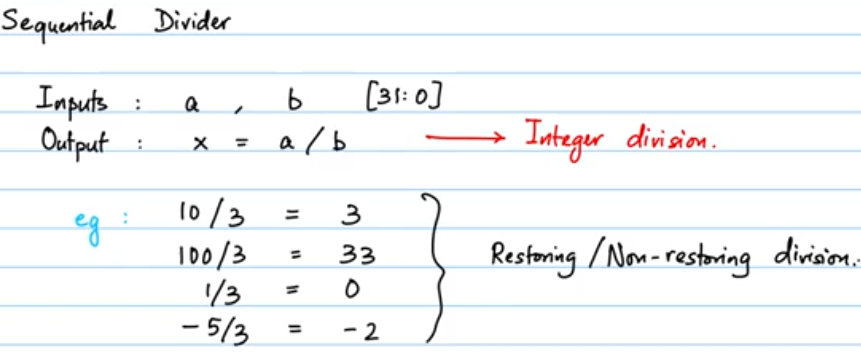
\includegraphics[scale=0.4]{Resources/Images/Assignment2_Desc.png}
\end{figure}


Method To Used:
\begin{itemize}
    \item Restoring/ Non-restoring Division
\end{itemize}


\subsection{Using Start and Stop Signal}
\begin{figure}[H]
    \centering
    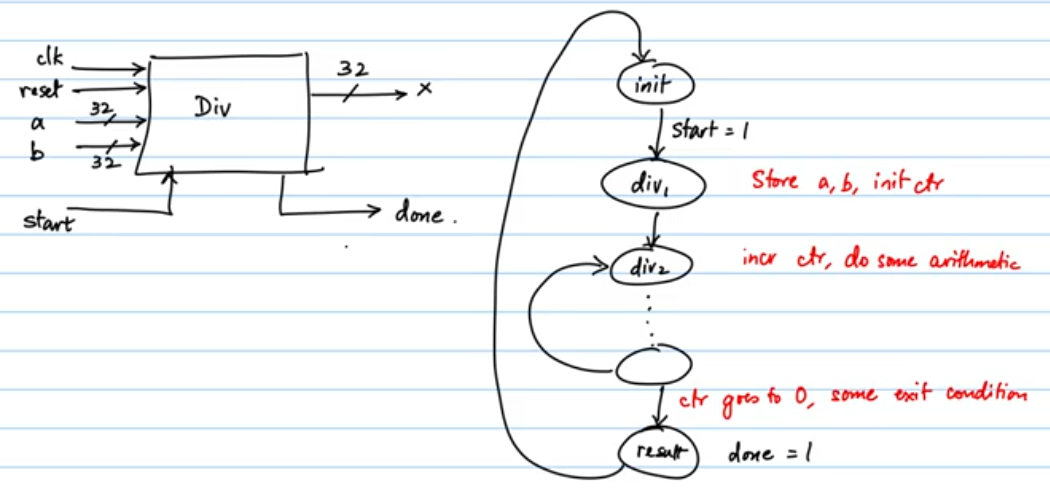
\includegraphics[scale=0.3]{Resources/Images/Assignment2_IM1.png}
\end{figure}

\begin{itemize}
    \item IntegerDivision/RestoringDivisonV1/ for unsigned restoring division.
    \item IntegerDivision/NonRestoringDivisionV1/ for unsigned non-restoring division
    \item IntegerDivision/RestoringDivisionV2/ for signed restoring division.
    \item IntegerDivision/NonRestoringDivisionV2/ for signed non-restoring division
\end{itemize}

\subsection{Using ready and valid Signal}
\begin{figure}[H]
    \centering
    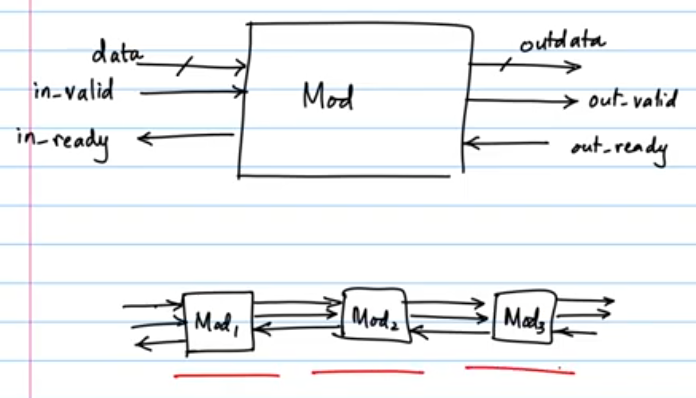
\includegraphics[scale=0.3]{Resources/Images/Assignment2_IM2.png}
\end{figure}
Done : See - IntegerDivision/IntegerDivisionWithValidReady

\subsection{Resources USed}
\begin{itemize}
    \item \href{https://web.stanford.edu/class/ee486/doc/chap5.pdf}{stanford}
    \item \href{https://www.youtube.com/watch?v=6ToR6vuRb3M}{Youtube link}
    \item \href{https://www.researchgate.net/publication/319302625_Hardware_implementation_of_methodologies_of_fixed_point_division_algorithms}{Signed Divison}
\end{itemize}


Finished On: \date{20-06-2021}

\end{document}